\subsubsection{ASTERIX Configuration}
\label{sec:configure_asterix_decoding}

The 'ASTERIX Configuration' leaf in the tree opens the per-category ASTERIX decoding settings of the active Data Context. \\

\begin{figure}[H]
  \centering
  \hspace*{-1cm}
    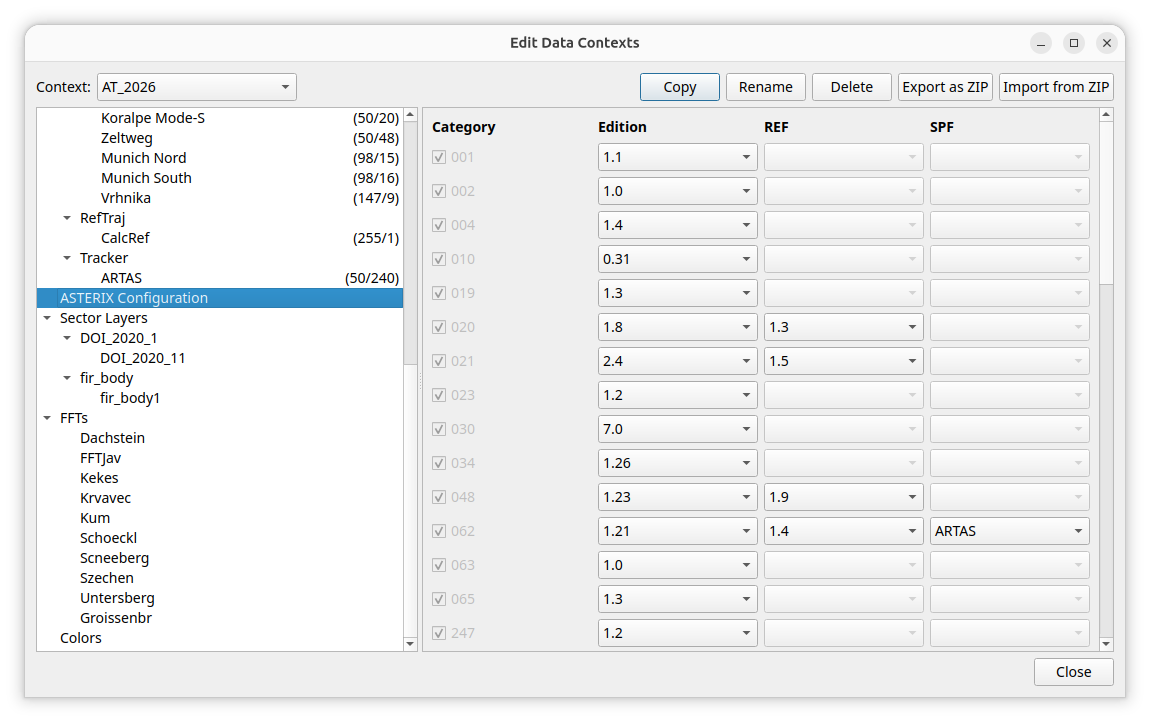
\includegraphics[width=17cm]{figures/data_context_edit_asterix.png}
  \caption{Data Context: ASTERIX Configuration widget}
\end{figure}

The decoding settings select, per ASTERIX Category, which Edition is used by the jASTERIX library to decode incoming target reports. They are stored as part of the active context and apply to all ASTERIX imports performed while the context is active. \\

For each defined category the widget shows the following columns:

\begin{itemize}
\item Category: ASTERIX category number (e.g. '001', '021', '048', '062')
\item Edition: Edition used to decode the main record
\item REF: Reserved Expansion Field (REF) edition, where applicable
\item SPF: Special Purpose Field (SPF) edition, where applicable
\end{itemize}
\ \\

The Edition, REF and SPF selectors are combo boxes pre-populated with the editions known to jASTERIX. Changing any value is stored immediately in the active context. \\

Please \textbf{note} that the same ASTERIX Configuration widget is also embedded into the ASTERIX import dialog, where the per-category enable/disable check boxes are editable (see \nameref{sec:ui_import_asterix}). When opened from the Data Context dialog, the check boxes serve as a read-only overview of the categories defined for the context. \\
